% ----------------------------------
% Cap Diseño
% ----------------------------------
%	Incluye
%		Diseño de interfaces y prototipos
%	    
%
\documentclass[a4paper,oneside,11pt]{book}

\usepackage[spanish,activeacute]{babel}
\usepackage[utf8]{inputenc}
%\usepackage[T1]{fontenc}
\usepackage{tabulary}
\usepackage{graphicx}
\usepackage{color}
\usepackage{float}

\setcounter{secnumdepth}{3}

\oddsidemargin=0.2cm
\headsep=1cm
\textheight=21cm
\textwidth=16cm

% Personalizamos la separación entre párrafos...
\parskip=6pt

% Personalizamos el identado en la primera línea del nuevo párrafo...
\parindent=10pt




\definecolor{gris}{gray}{0.80}
\definecolor{gris2}{gray}{0.90}
\definecolor{negro}{gray}{0}

\begin{document}
% cuerpo del documento
\title{Componentes}
\author{Pablo Eduardo Ojeda Vasco}
\date{\today}



	\maketitle
%
% Capítulo Diseño de interfaz de usuario
%
\chapter{Diseño} % (fold)
	\label{sec:diseno}

	\section{Diseño a nivel de componentes} % (fold)
	\label{sec:componentes}
	
	% section diseño_de_la_interfaz_de_usuario (end)
	\subsection{Introducción} % (fold)
		\label{sub:comp_introduccion}
	
		El diseño a nivel de componentes define las estructuras de los datos, los algoritmos, las características de la interfaz y los mecanismos de comunicación asignados a cada componente. Son muy importantes puesto que representan un nivel en el que es posible revisar los detalles y evaluar la calidad. Se utilizan diversos tipos de diagramas UML para representarlos.
		
		Desde la perspectiva del diseño orientado a objetos, podemos definir  un componente como un bloque que contiene un conjunto de clases que colaboran entre sí, en el cuál las clases tienen todos los atributos y operaciones relevantes para su implementación.
		
		El proceso que seguiremos acabo para diseñar el nivel de componentes será:
		\begin{itemize}
			\item A partir del modelo del análisis se elaborarán las clases de análisis y las de infraestructura, con sus principales atributos y métodos.
			\item Se diseñará el detalle algorítmico para la implementación de la lógica de las operaciones así como los mecanismos de las interfaces para la descripción de todos los mensajes que se requieran, lo cuál se hará mediante los diagramas de secuencia.
		\end{itemize}
	
	% subsection introduccion (end)
	
	\subsection{Diagrama de clases} % (fold)
		\label{sec:diagrama_de_clases}

			Un \textbf{diagrama de clases} es un tipo de diagrama estático que describe la estructura de un sistema mostrando sus clases, atributos y las relaciones entre ellos. Los diagramas de clases son utilizados durante el proceso de análisis y diseño de los sistemas, donde se crea el diseño conceptual de la información que se manejará en el sistema, y los componentes que se encargaran del funcionamiento y la relación entre uno y otro.

			Existen una serie de conceptos que tenemos que tener bastante claros. En primer lugar las \textbf{propiedades también llamados atributos o características}, son valores que corresponden a un objeto, como color, material, cantidad, ubicación. Generalmente se conoce como la información detallada del objeto. Suponiendo que el objeto es una puerta, sus propiedades serían: la marca, tamaño, color y peso.	El siguiente concepto son las \textbf{operaciones comúnmente llamados métodos}, son aquellas actividades o verbos que se pueden realizar con/para este objeto, como por ejemplo abrir, cerrar, buscar, cancelar, acreditar, cargar. De la misma manera que el nombre de un atributo, el nombre de una operación se escribe con minúsculas si consta de una sola palabra. Si el nombre contiene más de una palabra, cada palabra será unida a la anterior y comenzará con una letra mayúscula, a excepción de la primera palabra que comenzará en minúscula. Por ejemplo: abrirPuerta, cerrarPuerta, buscarPuerta, etc. Otro concepto es el de \textbf{interfaz}, que es un conjunto de operaciones que permiten a un objeto comportarse de cierta manera, por lo que define los requerimientos mínimos del objeto. Hace referencia a polimorfismo. Y por último el concepto de \textbf{herencia}, que se define como la reutilización de un objeto padre ya definido para poder extender la funcionalidad en un objeto hijo. Los objetos hijos heredan todas las operaciones y/o propiedades de un objeto padre. Anotar que los atributos y los métodos pueden ser privados, públicos o protegidos, permitiendo así ser accedidos o no por objetos de su misma o de otras clases. 

			Debemos tener conocimiento, además, de que a la hora de diseñar se suelen utilizar \textbf{patrones de diseño}, los cuales brindan una solución ya probada y documentada a problemas de desarrollo de software que están sujetos a contextos similares. Debemos tener presente los siguientes elementos de un patrón: su nombre, el problema (cuando aplicar un patrón), la solución (descripción abstracta del problema) y las consecuencias (costos y beneficios).

			El proyecto que nos atañe se basa en el \textit{framework rails}, que corre en el lenguaje de programación \textit{ruby}. \textit{Ruby on Rails} se basa en el patrón de diseño\textbf{Modelo Vista Controlador (MVC)}, que es un patrón de arquitectura de software que separa los datos de una aplicación, la interfaz de usuario, y la lógica de control en tres componentes distintos. El patrón de llamada y retorno MVC (según CMU), se ve frecuentemente en aplicaciones web como la que nos ocupa, donde \textbf{la vista} es la página HTML y el código que provee de datos dinámicos a la página. \textbf{El modelo} es el Sistema de Gestión de Base de Datos y la Lógica de negocio, y \textbf{el controlador} es el responsable de recibir los eventos de entrada desde la vista. 	

			Muchos de los sistemas informáticos utilizan un Sistema de Gestión de Base de Datos para gestionar los datos: en líneas generales del MVC corresponde al modelo. La unión entre capa de presentación y capa de negocio conocido en el paradigma de la Programación por capas representaría la integración entre Vista y su correspondiente Controlador de eventos y acceso a datos, MVC no pretende discriminar entre capa de negocio y capa de presentación pero si pretende separar la capa visual gráfica de su correspondiente programación y acceso a datos, algo que mejora el desarrollo y mantenimiento de la Vista y el Controlador en paralelo, ya que ambos cumplen ciclos de vida muy distintos entre sí.

			Aunque se pueden encontrar diferentes implementaciones de MVC, el flujo que sigue \textit{rails} es el siguiente:

			\begin{figure}[H]
			  \centering
			    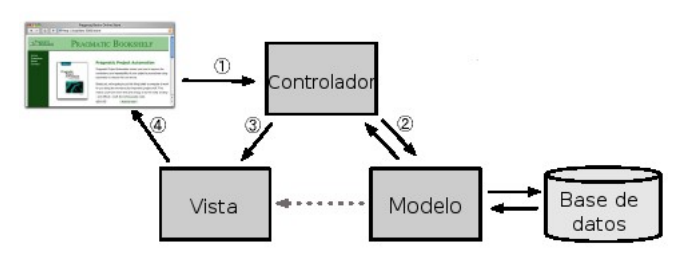
\includegraphics[width=16cm]{img/png/mvc.png}
			  \caption{Flujo Patrón Modelo Vista Controlador}
			  \label{fig:patron_mvc}
			\end{figure}

			\begin{enumerate}
				\item El usuario interactúa con la interfaz de usuario de alguna forma (por ejemplo, el usuario pulsa un botón, enlace, etc.). Entonces, el navegador envía una petición.
				\item El controlador recibe (por parte de los objetos de la interfaz-vista) la notificación de la acción solicitada por el usuario. El controlador gestiona el evento que llega. Entonces, el controlador accede al modelo (interactúa con el modelo), actualizándolo, posiblemente modificándolo de forma adecuada a la acción solicitada por el usuario (por ejemplo, el controlador actualiza los datos de un médico). Los controladores complejos están a menudo estructurados usando un patrón de comando que encapsula las acciones y simplifica su extensión.
				\item Los controladores invocan a las vistas.
				\item La vista \textit{dibuja} la siguiente página para el navegador.
				\item La interfaz de usuario espera nuevas interacciones del usuario, comenzando el ciclo nuevamente.
			\end{enumerate}

			A continuación el diagrama de clases (Figura \ref{fig:dis_clases}).

			\begin{figure}[H]
			  \centering
			    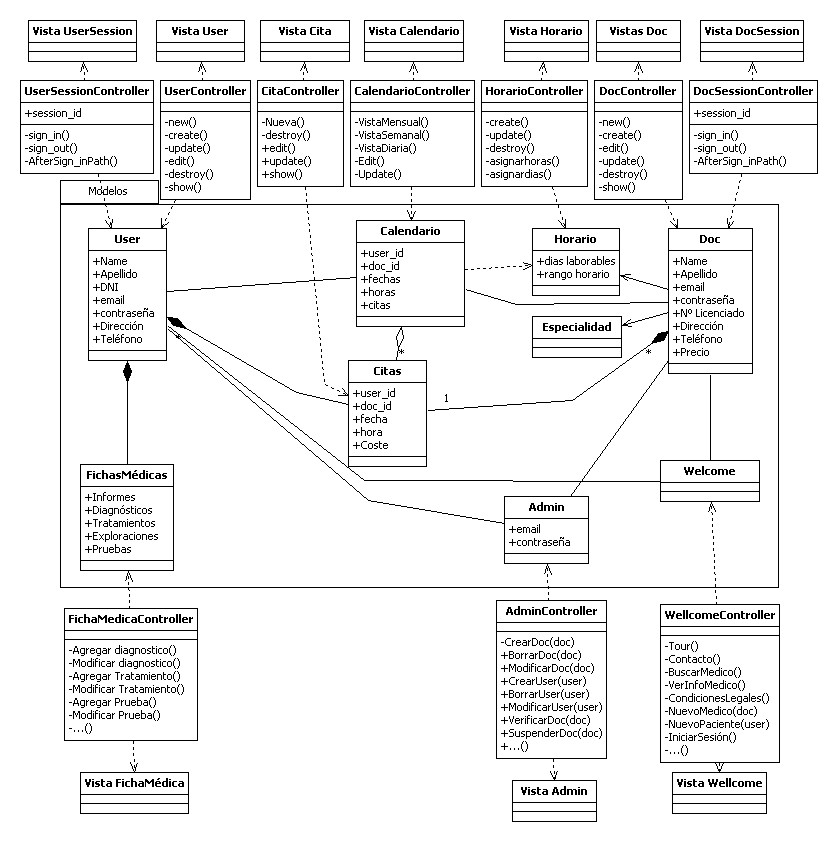
\includegraphics[width=16cm]{img/jpg/dis_clases/clases.jpg}
			  \caption{Diagrama de clases}
			  \label{fig:dis_clases}
			\end{figure}

	% section diagrama_de_clases (end)
	\newpage
	\subsection{Diagramas de secuencia} % (fold)
		\label{sec:diagramas_de_secuencia}

			Cómo fue explicado en capítulos anteriores, los diagramas de interacción son diagramas que describen cómo grupos de objetos colaboran para conseguir algún fin. Estos diagramas muestran objetos, así como los mensajes que se pasan entre ellos dentro del caso de uso, es decir, capturan el comportamiento de los casos de uso.

			Hay dos tipos de diagrama de interacción, ambos basados en la misma información, pero cada uno enfatizando un aspecto particular: \textbf{Diagramas de Secuencia} y Diagramas de Colaboración.

			\medskip

			\fcolorbox{negro}{gris}{\parbox{15cm}{Un \textit{diagrama de Secuencia} muestra una interacción ordenada según la secuencia temporal de eventos. En particular, muestra los objetos participantes en la interacción y los mensajes que intercambian ordenados según su secuencia en el tiempo. Es decir, muestra la interacción de un conjunto de objetos en una aplicación a través del tiempo y se modela para cada caso de uso.}}

			\medskip

			En cuanto a la \textbf{representación}, el eje vertical representa el tiempo, y en el eje horizontal se colocan los objetos y actores participantes en la interacción, sin un orden prefijado. Cada objeto o actor tiene una línea vertical, y los mensajes se representan mediante flechas entre los distintos objetos. El tiempo fluye de arriba abajo. Se pueden colocar etiquetas (como restricciones de tiempo, descripciones de acciones, etc.) bien en el margen izquierdo o bien junto a las transiciones o activaciones a las que se refieren. 

			En esta parte del diseño, al igual que en el resto del documento, vamos a dividir los diagramas de secuencia en cinco grandes grupos. Así, se detallan dos diagramas de secuencia hacen referencia a:
			\begin{itemize}
				\item Acciones generales.
				\item Médicos.
				\item Pacientes.
				\item Administrador.
				\item Fichas médicas.
			\end{itemize}
			

			\paragraph{Diagramas de secuencia de las Actividades Generales.} % (fold)
			\label{par:diagramas_de_secuencia_de_las_actividades_generales_}
			
				\subparagraph{Acceso y Autentificación} % (fold)
				\label{subp:cont_acceso_y_autentificacion}
				
					Gestionado por el controlador y las vistas de \textit{sessions} y haciendo uso del modelo \textit{user.}
					Si todo va correctamente, tal y como se muestra en la Figura \ref{fig:cont_user_login}, un usuario introducirá su email y su contraseña en la vista. El sistema (control) creará una nueva sesión si los datos son correctos. Además, en el diagrama se aprecia que se ha accedido con el rol de médico, y por tanto el controlador de sesión redirige al usuario al panel correspondiente.
					
					\begin{figure}[H]
					  \centering
					    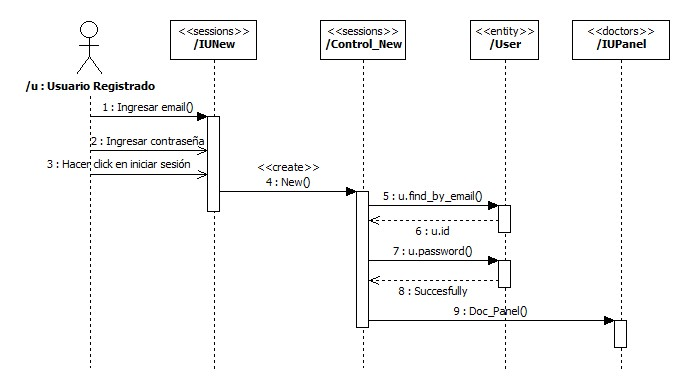
\includegraphics[width=14.5cm]{img/jpg/secuencia/18_user_login.jpg}
					  \caption{D. de secuencia del acceso y autentificación.}
					  \label{fig:cont_user_login}
					\end{figure}
				
				En el caso de que el email o la contraseña introducidos no sean correctos, o de que el usuario no exista (Figura \ref{fig:cont_user_login_error}), no se creará una nueva sesión, se renderizará de nuevo la vista de iniciar nueva sesión y se informará de que los datos introducidos no son correctos. Concretamente, en el diagrama se observa que el email introducido no existe.
				
					\begin{figure}[H]
					  \centering
					    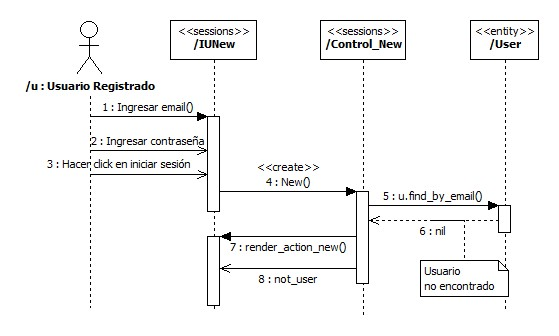
\includegraphics[width=12.5cm]{img/jpg/secuencia/19_user_login_error.jpg}
					  \caption{D. de secuencia de error en el acceso y autentificación.}
					  \label{fig:cont_user_login_error}
					\end{figure}
				
				Por último, podemos hacer que nuestro inicio de sesión sea recordado, para no tener que introducir los datos cada vez que accedemos a la aplicación desde el navegador. Para ello, tal y como se muestra en la Figura \ref{fig:cont_user_login_remember}, se utilizan las \textit{cookies} haciendo uso de un \textit{helper de rails}.
				
					\begin{figure}[H]
					  \centering
					    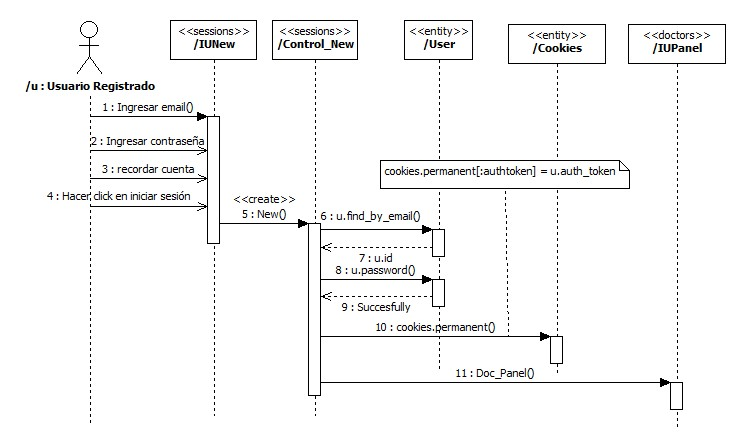
\includegraphics[width=16cm]{img/jpg/secuencia/20_user_login_remember.jpg}
					  \caption{D. de secuencia de recordar acceso y autentificación.}
					  \label{fig:cont_user_login_remember}
					\end{figure}
				
				% subparagraph acceso_y_autentificación (end)
			
				\subparagraph{Registro} % (fold)
				\label{subp:cont_registro}
				
					Se gestiona desde el controlador y las vistas \textit{users} y hace uso del modelo \textit{user}. Es el mismo tanto para médicos como para pacientes, excepto porque el valor \textit{rol} difiere en cada caso (\textit{doc} o \textit{patient}). Como vemos en el diagrama de la Figura \ref{fig:cont_user_new}, el usuario debe introducir el email, la contraseña y la confirmación de la contraseña. Todo será validado por el sistema. Si todo es correcto, se creará una nueva instancia de usuario con el rol que le corresponda. Además, se generará un \textit{authtoken}, que es un código único asociado a cada usuario para ser identificado en el caso de querer que se recuerde la sesión.
					
					Si se produjese un error, bien porque el formato de email es incorrecto, las contraseñas no coinciden o el usuario ya existe, simplemente se renderizará de nuevo la vista de nuevo usuario y se informará del error que se ha producido (Figura \ref{fig:cont_user_new_error})
					
					\begin{figure}[H]
					  \centering
					    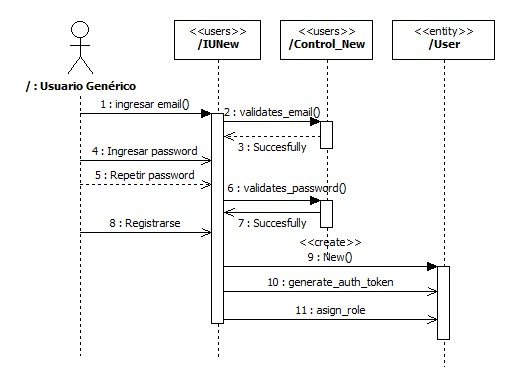
\includegraphics[width=13cm]{img/jpg/secuencia/21_user_new.jpg}
					  \caption{D. de secuencia de nuevo usuario.}
					  \label{fig:cont_user_new}
					\end{figure}

					\begin{figure}[H]
					  \centering
					    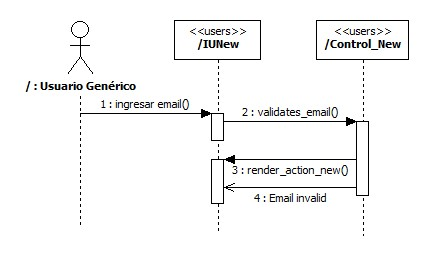
\includegraphics[width=10cm]{img/jpg/secuencia/22_user_new_error.jpg}
					  \caption{D. de secuencia de error en nuevo usuario.}
					  \label{fig:cont_user_new_error}
					\end{figure}
				% subparagraph registro (end)
				\newpage
				\subparagraph{Buscar Médico} % (fold)
				\label{subp:cont_buscar_medico}
					
					Utiliza el controlador y las vistas del \textit{welcome} y el modelo \textit{user}. Realiza una búsqueda en la base de datos en función del filtro seleccionado y los campos que se desean buscar. Finalmente se muestra una vista con la lista de los resultados al usuario (Figura \ref{fig:cont_user_search_doc}). En el caso de no encontrar resultados, simplemente se mostrará la vista informando de que no existen elementos para la búsqueda realizada.
					
					\begin{figure}[H]
					  \centering
					    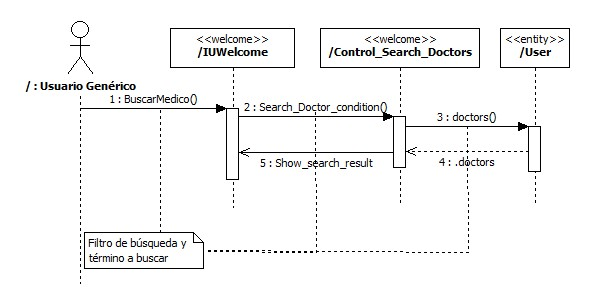
\includegraphics[width=12cm]{img/jpg/secuencia/24_user_search_doc.jpg}
					  \caption{D. de secuencia de buscar médico.}
					  \label{fig:cont_user_search_doc}
					\end{figure}
					
				% subparagraph buscar_médico (end)
				
				\subparagraph{Tour y resto de actividades} % (fold)
				\label{subp:tour_y_resto_de_actividades}
				
					Harán uso del controlador y vistas del \textit{welcome}, y de las entidades del \textit{tour, datos de contacto, términos legales, condiciones de uso}. En el diagrama de la Figura \ref{fig:cont_user_tour} se puede observar como el usuario selecciona la acción de \textit{ver tour}, el controlador busca en la entidad \textit{tour} la información y renderiza la vista correspondiente con dichos datos. El resto de acciones son exactamente igual, simplemente que se accede a la entidad correspondiente y se muestra la vista adecuada.
					
					\begin{figure}[H]
					  \centering
					    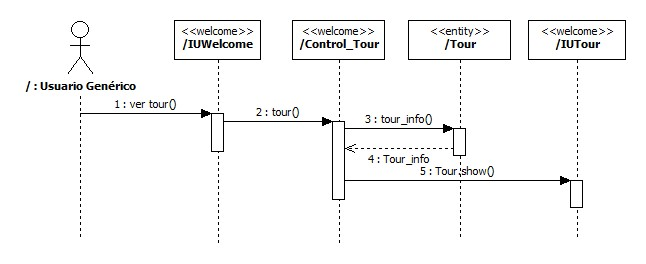
\includegraphics[width=13cm]{img/jpg/secuencia/23_user_tour.jpg}
					  \caption{D. de secuencia ver tour.}
					  \label{fig:cont_user_tour}
					\end{figure}
				
				% subparagraph tour_y_resto_de_actividades (end)
			% paragraph diagramas_de_secuencia_de_las_actividades_generales_ (end)
			
			
			\paragraph{Diagramas de secuencia de los Médicos.} % (fold)
			\label{par:diagramas_de_secuencia_de_los_medicos_}
			
				\subparagraph{Configuración del médico} % (fold)
				\label{subp:cont_configuracion_doc}
				
					Utilizará las vistas y el controlador \textit{doctors}, y el modelo \textit{user, schedule y notification.}
					
					En primer lugar vemos la configuración de los datos personales (Figura \ref{fig:cont_doc_config_data}). En ella, el usuario introduce los datos personales, de contacto y de localización en las vistas. El controlador verificará la información, y si todo es correcto, se actualizarán los atributos del médico correspondiente y se informará de que todo ha ido correctamente. En caso de que se produzca algún error, se notificará al usuario y se renderizará de nuevo la vista de la edición de datos.
					
					\begin{figure}[H]
					  \centering
					    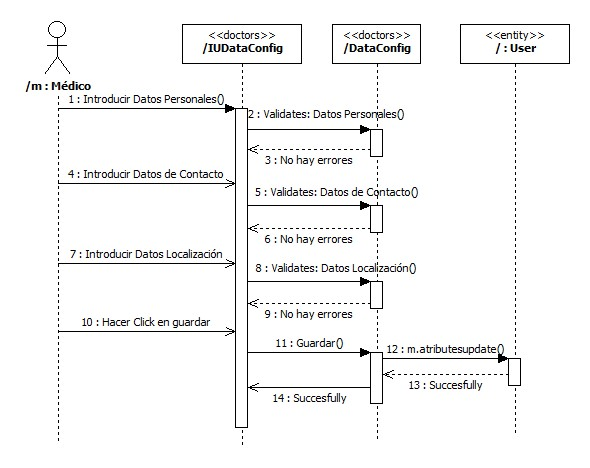
\includegraphics[width=14cm]{img/jpg/secuencia/1_doc_config_data.jpg}
					  \caption{D. de secuencia de configuración de datos del médico.}
					  \label{fig:cont_doc_config_data}
					\end{figure}
					
					La configuración de la cuenta es muy similar. En este, el diagrama de la Figura \ref{fig:cont_doc_config_account} muestra como se modifica la contraseña. Modificar el email o el idioma es igual, simplemente que no es necesario repetirlo, como ocurre con la contraseña. Si no existen errores, se actualizan los atributos del usuario y se informa. En caso contrario, se notificará y se volverá a la vista de edición de cuenta.
					
					\begin{figure}[H]
					  \centering
					    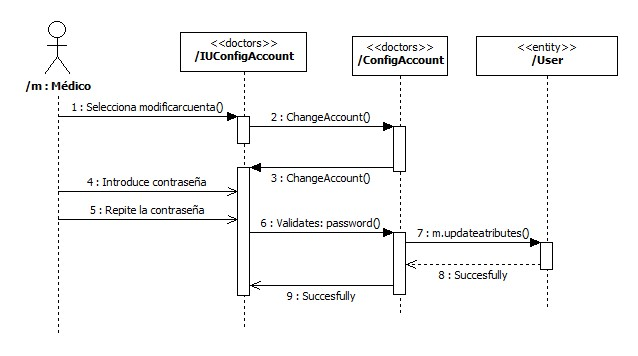
\includegraphics[width=14cm]{img/jpg/secuencia/2_doc_config_account.jpg}
					  \caption{D. de secuencia de configuración de cuenta del médico.}
					  \label{fig:cont_doc_config_account}
					\end{figure}
				
				\begin{figure}[H]
				  \centering
				    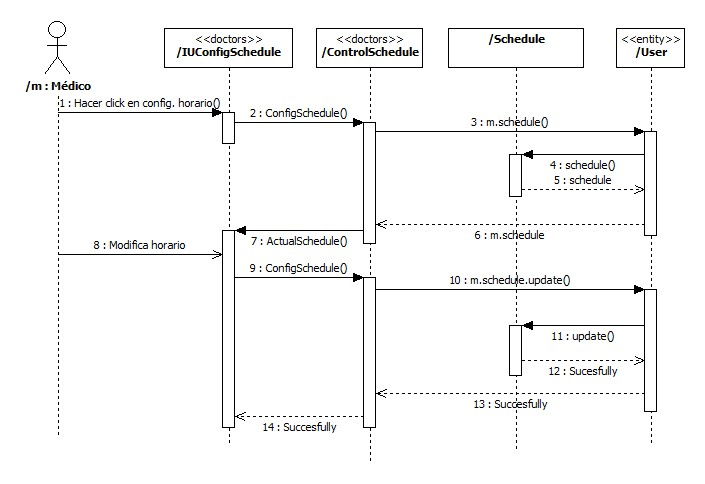
\includegraphics[width=15cm]{img/jpg/secuencia/3_doc_config_schedule.jpg}
				  \caption{D. de secuencia de configuración de horario del médico.}
				  \label{fig:cont_doc_config_schedule}
				\end{figure}
				
				En la configuración del horario (Figura \ref{fig:cont_doc_config_schedule}), el controlador \textit{doctors} busca en primer lugar en la tabla \textit{users} la configuración actual, que debe buscarla a su vez en la tabla \textit{schedules}. Una vez se tienen los datos necesarios, se muestra al usuario el formulario con la información actual para que este la modifique a su gusto. En la mayoría de los casos todo será correcto, se actualizará el médico (m) y su horario (schedule). En caso de existir cualquier error, simplemente se notificará y se renderizará la vista de modificar horario.
				
				La configuración de las notificaciones es igual que la del horario, simplemente que la información se buscará y se actualizará en las notificaciones del médico correspondiente (m).
				% subparagraph configuración (end)
			
				\subparagraph{Calendario del médico} % (fold)
				\label{subp:cont_calendario}
				
					En lo referente a los calendarios del médico, estaremos siempre trabajando con el controlador y las vistas de \textit{doctors} y con los modelos \textit{user, schedule y event}.
					
					Principalmente podemos ver tres tipos de vista: diaria, semanal y mensual. En el diagrama de la Figura \ref{fig:cont_doc_calendar} vemos la vista semanal. Para mostrarla, el controlador busca en el usuario su calendario mediante su horario (Schedule) y sus citas (Event), para mostrar una vista dividida en franjas horarias en función de su horario de trabajo y que aparezcan las citas que ya tiene concertadas. Si todo ha ido correctamente, el médico verá su agenda semanal. Lo mismo ocurre con las otras funciones (diaria y mensual), cambiando la vista que se presenta al usuario.
					
					\begin{figure}[H]
					  \centering
					    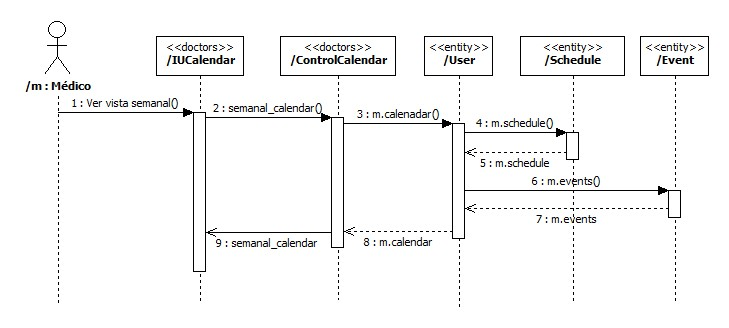
\includegraphics[width=16cm]{img/jpg/secuencia/4_doc_calendar_semanal.jpg}
					  \caption{D. de secuencia de vista semanal del médico.}
					  \label{fig:cont_doc_calendar}
					\end{figure}
					
					Otra acción importante es la de anular una cita (Figura \ref{fig:cont_doc_calendar_anular}), que se puede realizar bien desde la vista diaria, bien desde la semanal. Para ello, una vez seleccionada la cita a eliminar, se realiza un \textit{delete} de los eventos del usuario y de la tabla de eventos.
					
					\begin{figure}[H]
					  \centering
					    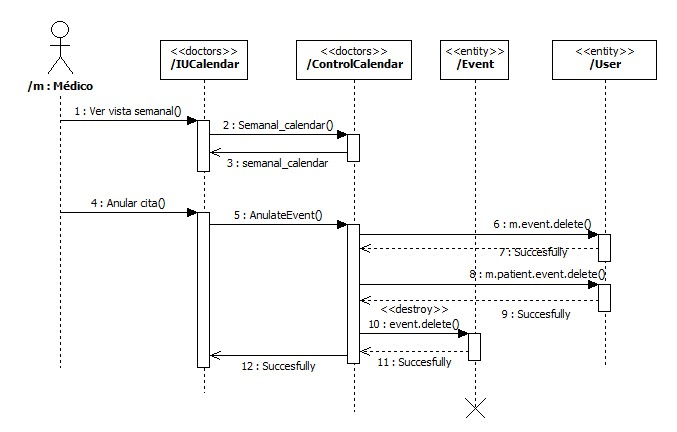
\includegraphics[width=14cm]{img/jpg/secuencia/5_doc_calendar_anular.jpg}
					  \caption{D. de secuencia de anular una cita.}
					  \label{fig:cont_doc_calendar_anular}
					\end{figure}
					
					Por su parte, anular un día entero es un bucle de anular las citas existentes en un día.
					
					
				% subparagraph calendario (end)
			
				\subparagraph{Pacientes del médico} % (fold)
				\label{subp:cont_pacientes_del_medico}
				
					Hace uso de las vistas y del controlador \textit{doctors} y de los modelos \textit{user, event y fichamedica}.
					
					Para ver todos los pacientes (Figura \ref{fig:cont_doc_patients}), simplemente tenemos que buscar los pacientes (\textit{users} con rol \textit{patient}) del médico \textit{m}. Si quisiéramos ver los próximos o los últimos pacientes, el procedimiento sería cargar la lista de citas del médico, y mostrar las próximas o las siguientes en función del momento actual. Es decir, sería igual que el diagrama de la Figura \ref{fig:cont_doc_patients}, pero buscando en la tabla \textit{events}.
					
					\begin{figure}[H]
					  \centering
					    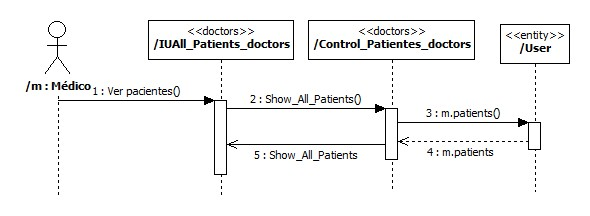
\includegraphics[width=11cm]{img/jpg/secuencia/7_doc_patients_all.jpg}
					  \caption{D. de secuencia de ver todos los pacientes del médico.}
					  \label{fig:cont_doc_patients}
					\end{figure} 
					
					Para buscar un paciente (Figura \ref{fig:cont_doc_patient_search}), debemos aplicar un filtro de búsqueda (nombre, diagnóstico, enfermedad, etcétera) y buscar en los pacientes del médico en función de los filtros y campos introducidos. Se mostrará la vista con los resultados. En caso de no existir ninguno, se notificará al usuario en la vista.
					
					\begin{figure}[H]
					  \centering
					    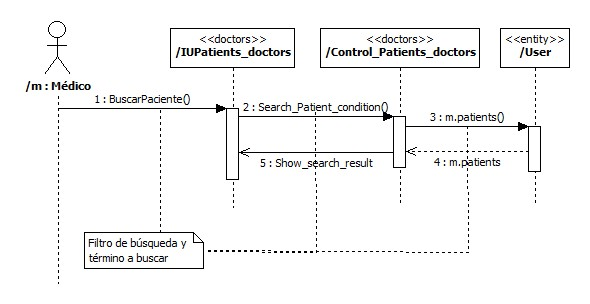
\includegraphics[width=13cm]{img/jpg/secuencia/8_doc_patients_search.jpg}
					  \caption{D. de secuencia de buscar pacientes del médico.}
					  \label{fig:cont_doc_patient_search}
					\end{figure}
				
				% subparagraph pacientes_del_médico (end)
				
				\subparagraph{Ver ficha médica} % (fold)
				\label{subp:cont_ver_ficha_medica}
					
						Para ver la ficha médica de un paciente, podemos hacerlo bien desde el calendario, bien desde la lista de pacientes del médico. En el diagrama de la Figura \ref{fig:cont_doc_ficha} lo hacemos después de buscar un paciente, y haciendo uso del controlador y las vistas \textit{doctors} y los modelos \textit{user y fichamedico}.
						
						\begin{figure}[H]
						  \centering
						    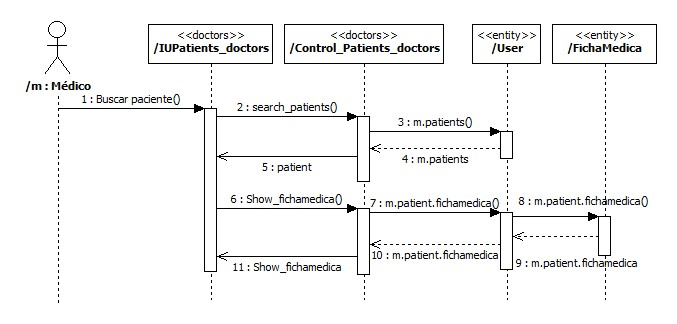
\includegraphics[width=14cm]{img/jpg/secuencia/6_doc_ver_ficha.jpg}
						  \caption{D. de secuencia de ver ficha médica.}
						  \label{fig:cont_doc_ficha}
						\end{figure}
				% subparagraph ver_ficha_médica (end)
				
			% paragraph diagramas_de_secuencia_de_los_médicos_ (end)

			
			\paragraph{Diagramas de secuencia de los Pacientes.} % (fold)
			\label{par:diagramas_de_secuencia_de_los_pacientes_}
			
				\subparagraph{Configuración del paciente} % (fold)
				\label{subp:cont_configuracion_paciente}
				
					Utilizará las vistas y el controlador \textit{patients}, y el modelo \textit{user y notification.}
					
					En primer lugar vemos la configuración de los datos personales (Figura \ref{fig:cont_patient_config_data}). En ella, el usuario introduce los datos personales y los de contacto en las vistas. El controlador verificará la información, y si todo es correcto, se actualizarán los atributos del paciente correspondiente y se informará de que todo ha ido correctamente. En caso de que se produzca algún error, se notificará al usuario y se renderizará de nuevo la vista de la edición de datos.
					
					\begin{figure}[H]
					  \centering
					    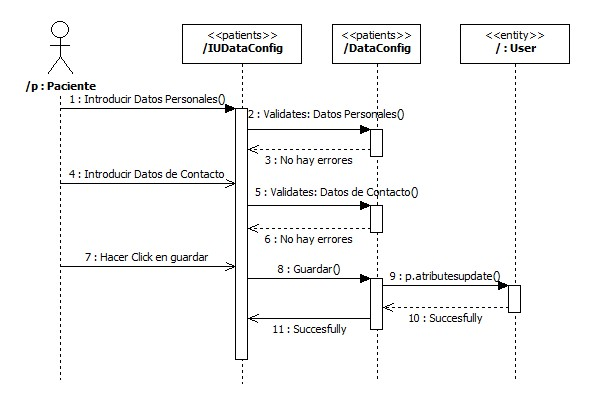
\includegraphics[width=14cm]{img/jpg/secuencia/14_patients_config_data.jpg}
					  \caption{D. de secuencia de configuración de datos del paciente.}
					  \label{fig:cont_patient_config_data}
					\end{figure}
					
					La configuración de la cuenta es muy similar. En este, el diagrama de la Figura \ref{fig:cont_patient_config_account} muestra como se modifica el idioma. Modificar el email o la contraseña es igual, simplemente que la contraseña es necesario repetirla. Si no existen errores, se actualizan los atributos del usuario y se informa. En caso contrario, se notificará y se volverá a la vista de edición de cuenta.
					
					\begin{figure}[H]
					  \centering
					    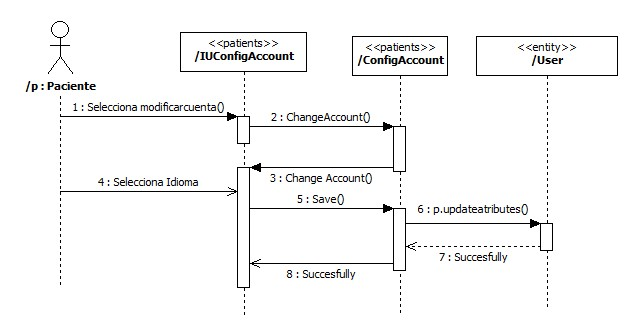
\includegraphics[width=14cm]{img/jpg/secuencia/15_patients_config_account.jpg}
					  \caption{D. de secuencia de configuración de cuenta del paciente.}
					  \label{fig:cont_patient_config_account}
					\end{figure}
				
				% subparagraph configuración (end)
			
				\subparagraph{Calendario del paciente} % (fold)
				\label{subp:cont_calendario_paciente}
				
					En lo referente a los calendarios del paciente, se hará uso del controlador y las vistas de \textit{patients} y con los modelos \textit{user y event}.
					
					Principalmente podemos ver tres tipos de vista: diaria, semanal y mensual. En el diagrama de la Figura \ref{fig:cont_patient_calendar} vemos la vista semanal. Para mostrarla, el controlador busca en el usuario (User) y sus citas (Event), para mostrar una vista dividida en franjas horarias en la que aparezcan las citas que ya tiene concertadas. Si todo ha ido correctamente, el paciente verá su agenda semanal. Lo mismo ocurre con las otras funciones (diaria y mensual), cambiando la vista que se presenta al usuario.
					
					\begin{figure}[H]
					  \centering
					    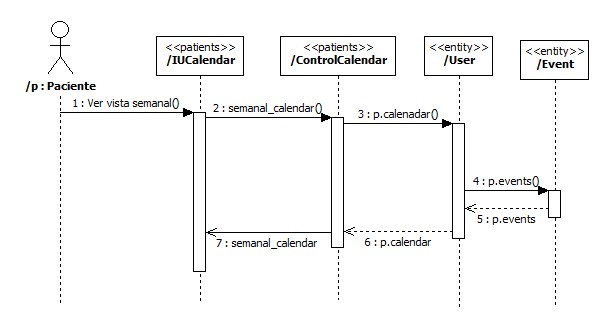
\includegraphics[width=13.5cm]{img/jpg/secuencia/9_patient_calendar_semanal.jpg}
					  \caption{D. de secuencia de vista semanal del paciente.}
					  \label{fig:cont_patient_calendar}
					\end{figure}
					
					Otra acción importante es la de anular una cita (Figura \ref{fig:cont_patient_calendar_anular}), que se puede realizar bien desde la vista diaria, bien desde la semanal. Para ello, una vez seleccionada la cita a eliminar, se realiza un \textit{delete} de los eventos del usuario y de la tabla de eventos.
					
					\begin{figure}[H]
					  \centering
					    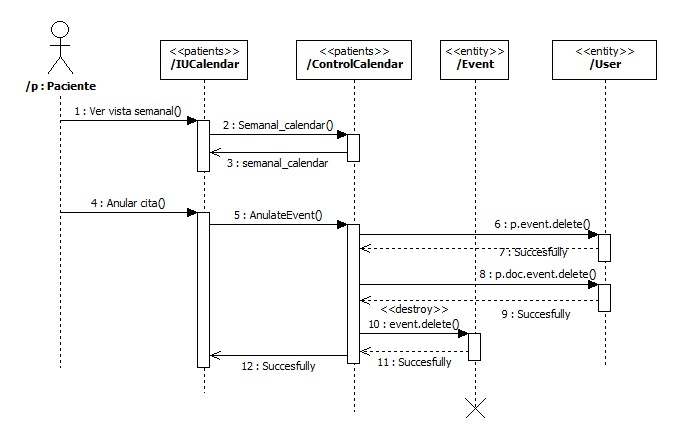
\includegraphics[width=13.5cm]{img/jpg/secuencia/10_patients_calendar_anular.jpg}
					  \caption{D. de secuencia de anular una cita.}
					  \label{fig:cont_patient_calendar_anular}
					\end{figure}
					
				% subparagraph calendario (end)
			
				\subparagraph{Médicos del paciente} % (fold)
				\label{subp:cont_medicos_del_paciente}
				
					Hace uso de las vistas y del controlador \textit{patients} y de los modelos \textit{user, event y fichamedica}.
					
					Para ver todos los médicos (Figura \ref{fig:cont_patient_docs}), simplemente tenemos que buscar los medicos (\textit{users} con rol \textit{doc}) del paciente \textit{p}. Si quisiéramos ver los próximos o los últimos médicos, el procedimiento sería cargar la lista de citas (Event) del paciente, y mostrar las próximas o las siguientes en función del momento actual. Es decir, sería igual que el diagrama de la Figura \ref{fig:cont_patient_docs}, pero buscando en la tabla \textit{events}.
					
					\begin{figure}[H]
					  \centering
					    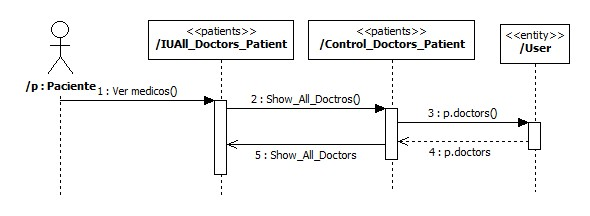
\includegraphics[width=11cm]{img/jpg/secuencia/12_patients_alll_doctors.jpg}
					  \caption{D. de secuencia de ver todos los médicos del paciente.}
					  \label{fig:cont_patient_docs}
					\end{figure} 
					
					Para buscar un médico (Figura \ref{fig:cont_patient_doc_search}), debemos aplicar un filtro de búsqueda (nombre, especialidad, localidad, etcétera) y buscar en los médicos del paciente en función de los filtros y campos introducidos. Se mostrará la vista con los resultados. En caso de no existir ninguno, se notificará al usuario en la vista.
					
					\begin{figure}[H]
					  \centering
					    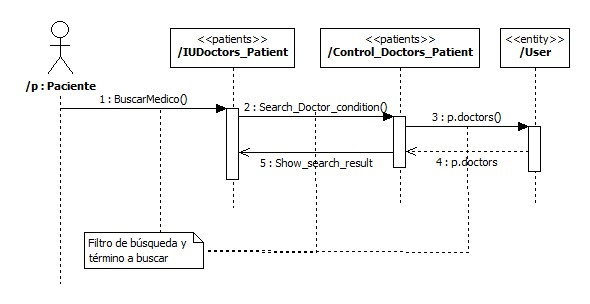
\includegraphics[width=13cm]{img/jpg/secuencia/13_patients_search_doctor.jpg}
					  \caption{D. de secuencia de buscar médicos del paciente.}
					  \label{fig:cont_patient_doc_search}
					\end{figure}
				
				% subparagraph pacientes_del_médico (end)
				
				\bigskip
				\bigskip		
				\subparagraph{Ver ficha médica} % (fold)
				\label{subp:cont_ver_ficha_medica2}
					
					En el diagrama de la Figura \ref{fig:cont_patient_ficha} hacemos uso del controlador y las vistas \textit{patients} y el modelo \textit{fichamedica}.
						
						\begin{figure}[H]
						  \centering
						    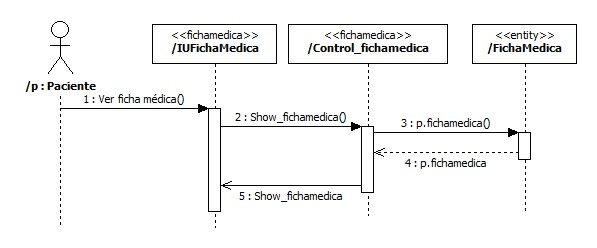
\includegraphics[width=14cm]{img/jpg/secuencia/11_patients_fichamedica.jpg}
						  \caption{D. de secuencia de ver ficha médica.}
						  \label{fig:cont_patient_ficha}
						\end{figure}
				% subparagraph ver_ficha_médica (end)
				
						
			% paragraph diagramas_de_secuencia_de_los_pacientes_ (end)


			\paragraph{Diagramas de secuencia del Administradores.} % (fold)
			\label{par:diagramas_de_secuencia_del_administradores_}
			
			
				\subparagraph{Respecto a los médicos} % (fold)
				\label{subp:cont_respecto_a_los_medicos}
				
					Se usarán el controlador y las vistas de \textit{admins} y los modelos \textit{user y notification}. Todos los casos de uso (verificar, suspender, reactivar y eliminar) son iguales, excepto que en eliminar se realiza un \textit{delete} del usuario (\textit{User}). Se puede ver en el diagrama de la Figura \ref{fig:cont_admin_verificate} que desde la vista se indica que se verifique el médico, y el controlador pondrá el estado del campo \textit{verificate} de dicho usuario (m) a activado. Luego se enviará la notificación correspondiente.
					
					\begin{figure}[H]
					  \centering
					    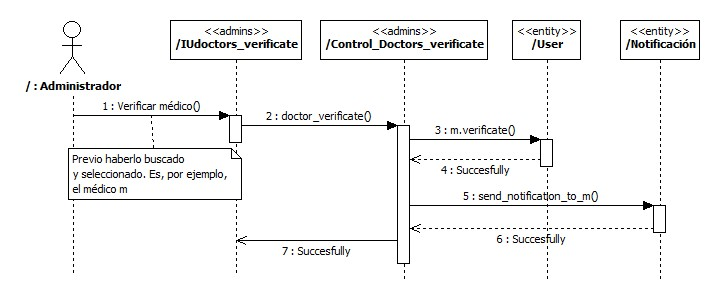
\includegraphics[width=15cm]{img/jpg/secuencia/16_admins_verificate.jpg}
					  \caption{D. de secuencia de verificación de médico.}
					  \label{fig:cont_admin_verificate}
					\end{figure}	
				
				% subparagraph respecto_a_los_médicos (end)
			
				\subparagraph{Respecto a la edición de información varia} % (fold)
				\label{subp:cont_respecto_a_la_edicion_de_informacion_varia}
				
					Se usarán el controlador y las vistas de \textit{admins} y los modelos \textit{user, conditions, terminoslegales, contacto, etcétera.}
					
					Todos los casos de uso utilizan un diagrama de secuencia muy similar, modificando cada uno de ellos la tabla que le corresponda con la información redactada. En el diagrama de la Figura \ref{fig:cont_admin_condition} podemos ver como se editan y actualizan las condiciones de uso.
					
					\begin{figure}[H]
					  \centering
					    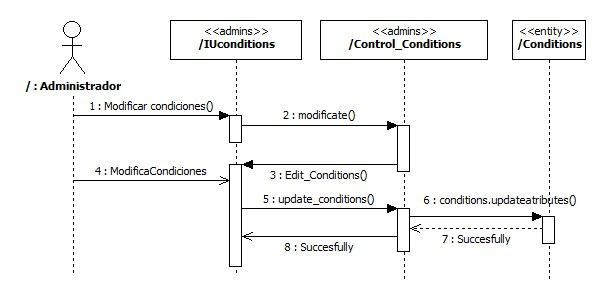
\includegraphics[width=14cm]{img/jpg/secuencia/17_admins_condition.jpg}
					  \caption{D. de secuencia de edición de las condiciones de uso.}
					  \label{fig:cont_admin_condition}
					\end{figure}
				
				
				% subparagraph respecto_a_la_edición_de_información_varia (end)
			% paragraph diagramas_de_secuencia_del_administradores_ (end)


			\paragraph{Diagramas de secuencia de las Fichas médicas.} % (fold)
			\label{par:diagramas_de_secuencia_de_las_fichas_medicas}
			
				Todos los diagramas de secuencia relacionados con las fichas médicas son muy similares. El motivo es que todos son casos C.R.U.D y sólo difieren en el tipo de objeto que se crea, se modifica, se visualiza o se elimina. Así, encontramos el controlador y las vistas \textit{fichamedica} y los modelos \textit{user, diagnosticos, antecedentes, tratamientos, informes, observaciones, pruebas, exploraciones y observaciones}.
				
				Los diagramas de las Figuras \ref{fig:cont_ficha_ant}, \ref{fig:cont_ficha_ant_new}, \ref{fig:cont_ficha_ant_edit} hacen referencia a los antecedentes, pero como se ha mencionado, serán los mismos para el resto de los apartados.
				
				Ver un antecedente (Figura \ref{fig:cont_ficha_ant}) es simplemente seleccionar en la vista el que nos interese, el controlador se encargará de buscar el antecedente del usuario y nos lo mostrará de nuevo en la vista.
				
				\begin{figure}[H]
				  \centering
				    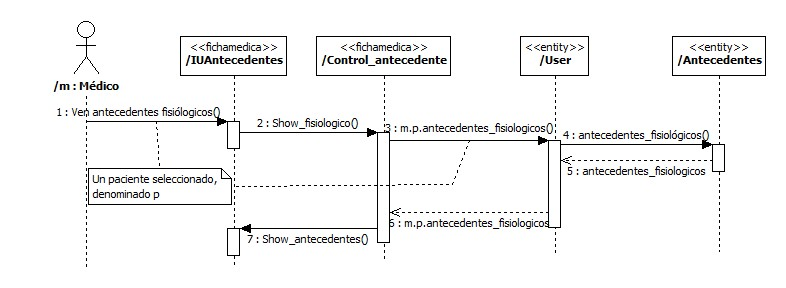
\includegraphics[width=16cm]{img/jpg/secuencia/25_ficha_showanteced.jpg}
				  \caption{D. de secuencia de ver un antecedente.}
				  \label{fig:cont_ficha_ant}
				\end{figure}
			
			Crear un nuevo antecedente es algo más complejo. En primer lugar se indica que se desea añadir un nuevo antecedente. A continuación, se muestra la vista correspondiente con el formulario. Una vez completo, el controlador hará un \textit{create} del nuevo antecedente y se lo asignará al usuario actualizando su información.
			
				\begin{figure}[H]
				  \centering
				    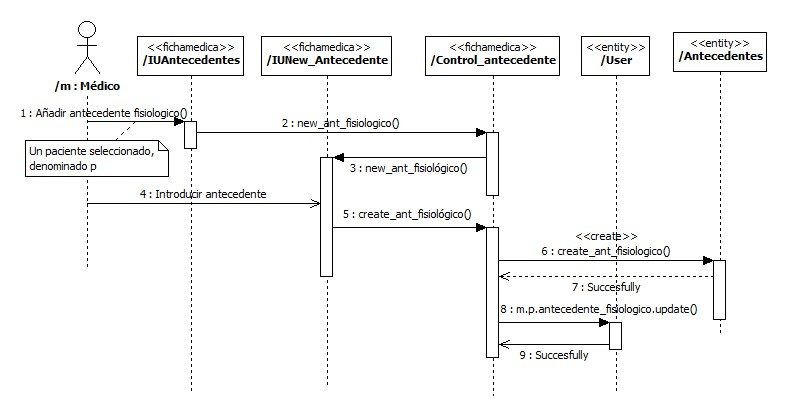
\includegraphics[width=16cm]{img/jpg/secuencia/26_ficha_new_ant.jpg}
				  \caption{D. de secuencia para añadir un nuevo antecedente.}
				  \label{fig:cont_ficha_ant_new}
				\end{figure}
			
			Por último vemos el diagrama de secuencia para modificar un antecedente. En primer lugar se selecciona el antecedente en la vista y se indica que vamos a editarlo. El controlador muestra la vista adecuada con el formulario para modificar la información. Por último, se actualizará el antecedente y la información del usuario.
			
				\begin{figure}[H]
				  \centering
				    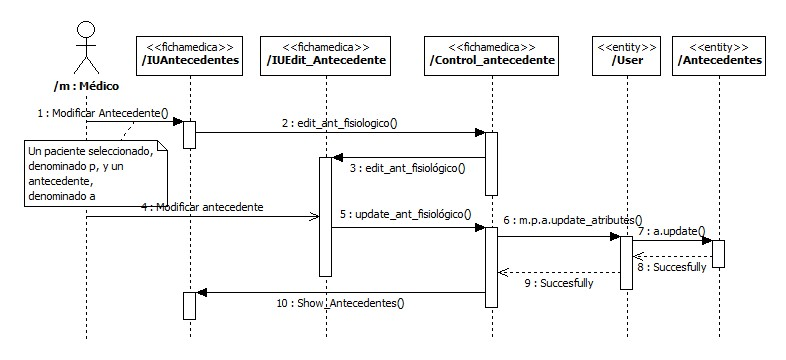
\includegraphics[width=16cm]{img/jpg/secuencia/27_ficha_edit_ant.jpg}
				  \caption{D. de secuencia para modificar un antecedente.}
				  \label{fig:cont_ficha_ant_edit}
				\end{figure}
			
			% paragraph diagramas_de_secuencia_de_las_fichas_médicas (end)

			% subsection actividades_generales (end)

	% section diagramas_de_secuencia (end)
	
	
	% section componentes (end)

\end{document}
% chapter diseño (end)